\chapter{Deep learning}
\section{Success stories}
We start this section introducing the two fields that have been spearheading the Deep Learning revolution: computer vision and speech recognition.
The first consists in identifying objects in digital images; while the second is being able to transcribe and process audio.

It is striking that both cases correspond to tasks that humans are very good at.
Indeed, neural networks are very good at \emph{perceptual learning}, or tasks where the computer replaces the human senses.
This is perhaps due to the fact that neural networks are inspired by the biological nervous system, but also because humans can understand the process,
label more data, and guess at why it is wrong.

But not only.
Deep neural networks have shown to be good at tasks that humans cannot perform well, like contact prediction~\citep{ultra_deep_contacts}, estimation of protein model quality~\citep{casp13_ema}, and other tasks.

%The rest of this chapter will contain a summary of the fundamental blocks, how to train, 

\section{The basic blocks}
A deep learning model is composed by a series of layers, or simple transformations (usually linear), plus a point-wise non-linearity.


\subsection{Fully connected layers}
Also known as ``dense" layers, they are the simplest building block of deep learning: a simple matrix multiplication, as described in the Section~\ref{sec:mlp}.
To make them more general, they can include a \emph{bias} term, that is added after the multiplication.

\begin{equation*}
\vec{o} = W \cdot \vec{i} + \vec{b}
\end{equation*}

Every element of the output is a function of every input, so this layer destroys the structure of the data.
On the other hand, since the intermediate layers can be arbitrarily large, it can have a lot of parameters, ie, it can be very expressive.
It is often used as the last layer of the model.

\subsection{Convolutions}
Convolutions capture spatial relationships in the data.
\todo{todo}

\subsection{Recurrent}
A recurrent layer tries to capture temporal dependencies on arbitrary time steps, such as those of natural language, or repeating motifs in proteins.
They work by taking two inputs: the vector at the current position, and the hidden state of the previous cell.
A simple cell:

\todo{todo}

\subsection{Non-linearities}
The workhorse of deep learning layers are linear transformations.
The composition of linear transformations is also linear, so in order to rip the benefits of multiple layers we need non-linearities.
For the most part, they are point-wise functions that act on the output of a layer.
Historically, the first non-linearity used was the sigmoid:

\begin{equation*}
f(x) = \frac{1}{1 + e^{- x}}
\end{equation*}

It has the advantage of clipping the range of values between 0 and 1, which makes the network stable with respect to large intermediate values (Figure~\ref{subfig:sigmoid}).
An improvement was the hyperbolic tangent:

\begin{equation*}
f(x) = \tanh(x) = \frac{e^x - e^{-x}}{e^x + e^{-x}},
\end{equation*}
with a similar shape to the sigmoid, but now outputting values between -1 and 1. (Figure~\ref{subfig:tanh})
Being anti-symmetric, it can achieve a stable distribution of outputs with normally weights in the intermediate layers.

\begin{figure}[tb]
	\subcaptionbox{Sigmoid\label{subfig:sigmoid}}{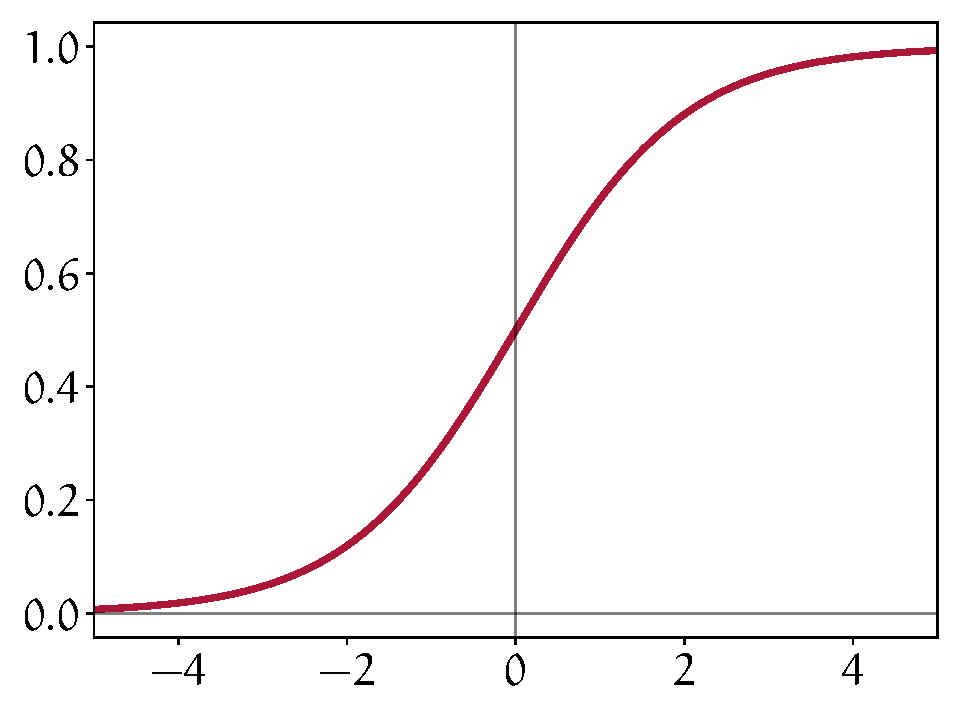
\includegraphics[width=0.45\textwidth]{machine_learning/figures/sigmoid}}
	\hfil
	\subcaptionbox{Tanh\label{subfig:tanh}}{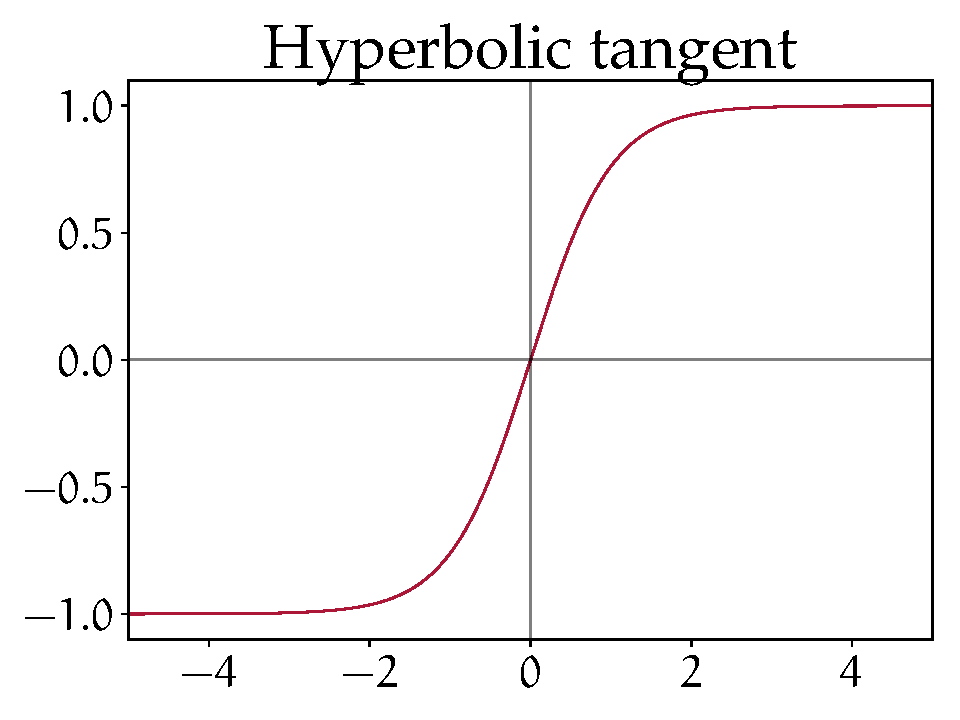
\includegraphics[width=0.45\textwidth]{machine_learning/figures/tanh}}
	\caption{Saturating non-linarities}\label{fig:non_linear}
\end{figure}

Both functions saturate on extreme values, \marginpar{Gradient saturation}
so their derivative approaches zero, which on one hand is useful to control the stability of the outputs, but on the other is a problem for the propagation of gradients.
The alternative is using non-saturating functions, that allow the gradients to flow for a wider range of values.

The simplest is the Rectified Linear Unit, or ReLU, introduced by~\citet{relu} and plotted in the Figure~\ref{subfig:relu}:
\begin{equation*}
f(x) =  \begin{cases}
\hfil x &  \text{if } x \geq 0 \\
\hfil 0 & otherwise
\end{cases}
\end{equation*}

But in this thesis I have mostly used the Exponential Linear Unit, or ELU, shown in the Figure~\ref{subfig:elu}:
\begin{equation*}
f(x) =  \begin{cases}
\hfil x &  \text{if } x \geq 0 \\
\frac{1}{1 + e^{-x}} & otherwise
\end{cases}
\end{equation*}

The choice of this non-linearity usually incurs in a slightly larger computational time for training, but a moderate improvement in performance as well.

\begin{figure}[tb]
	\subcaptionbox{ReLU\label{subfig:relu}}{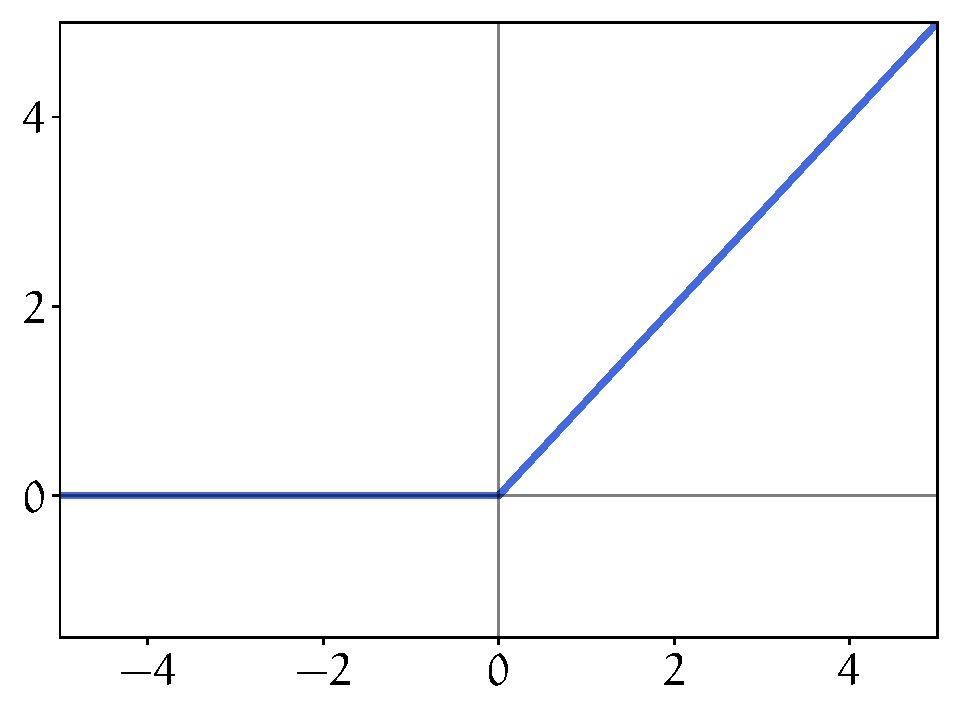
\includegraphics[width=0.45\textwidth]{machine_learning/figures/relu}}
	\hfil
	\subcaptionbox{ELU\label{subfig:elu}}{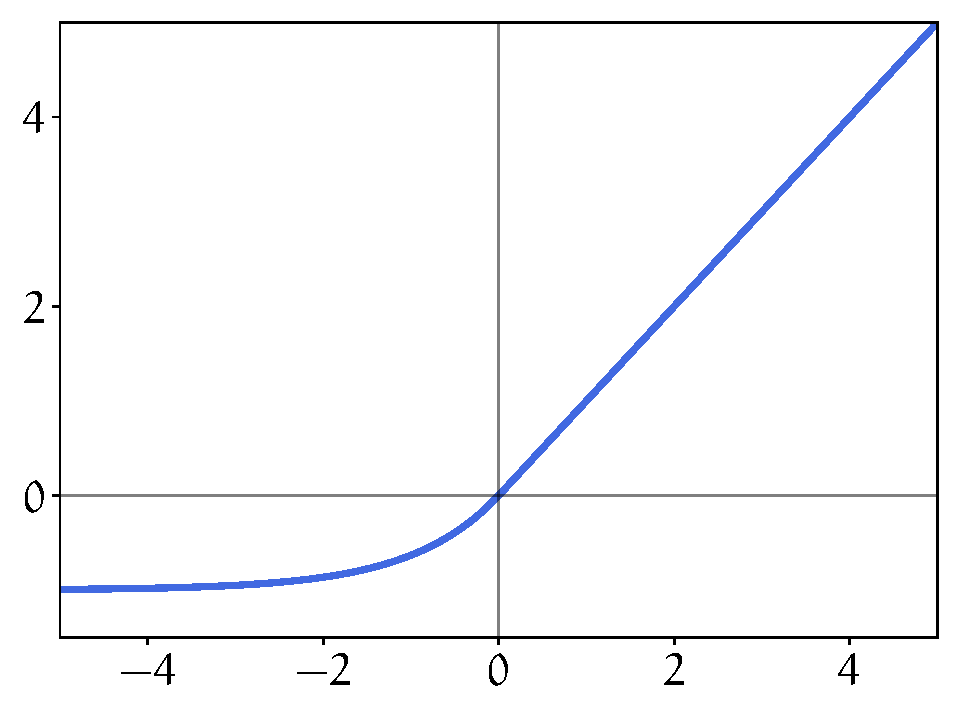
\includegraphics[width=0.45\textwidth]{machine_learning/figures/elu}}
	\caption{Non-saturating non-linarities}\label{fig:non_linear2}
\end{figure}

The last layer is an exception.\marginpar{Output}
The function applied depends on the properties of the target.
\begin{itemize}
\item If the output is a binary classification, or multiple mutually compatible classes, use a sigmoid, as described in the Section~\ref{sec:logistic_regression} on logistic regression.
\item If the output are a series of mutually exclusive classes, use a softmax, as explained in the Section~\ref{sec:mlp} on multi layered perceptrons.
\item If the output is a regression, use a linear layer to minimise the squeezing of the outputs.
This is valid even if the output is bounded between 0 and 1, when the values at the extrema are likely to appear, because the network would need to learn very high values for the logits.
\item If the outputs are angles, split the labels into sines and cosines and use the hyperbolic tangent.
This representation preserves angular distances (ie, angles that differ by almost $2 \pi$ are close), and are not biased towards an arbitrary middle point.
The original angle can be recovered using the $\arctantwo$ function.
\end{itemize}

\section[Gradient descent]{Training procedure: gradient descent}\label{sec:grad_descent}
A deep learning network can have millions of parameters, but how do we find the optimal values?

In the first place, we need to define a loss function, or a measurement of how wrong our predictions are on known data.
For example, the mean squared error for $N$ data points  $x_i$ with labels $y_i$ and predictions $o_i$ is:

\begin{equation*}
L_{MSE} = \sum_i^N \left(y_i - o_i\right)^2
\end{equation*}
and the cross entropy loss:
\begin{equation*}
L_{H} = \sum_i^N y_i \cdot \log\left(o_i\right) 
\end{equation*}

We initialise the network with random numbers, and measure how wrong we are.
Then, we compute the gradients of the loss with respect to each of the parameters $w_j$ of the network:
\begin{equation*}
g_j = \frac{1}{N}\sum_i^N\frac{\partial L\left(o_i, y_i \right)}{\partial w_j}
\end{equation*}

The gradients tell us in which direction we have to ``nudge" the network to improve its performance for the next iteration:

\begin{equation*}
\left. w_j\right|_{it=k+1} = \left. w_j\right|_{it=k} - \eta \cdot \left. g_j\right|_{it=k},
\end{equation*}
where $\eta$ is the step size, a small number that reflects our believe of the size of the region where the gradients still point in the same direction.

\subsection{Back-propagation}
In order to train, we need to compute the gradients of the loss with respect to all the parameters of the network.
This can be done automatically using the back-propagation algorithm, or \emph{backprop} \citep{backprop}, the machine version of the chain rule.

We start computing the derivative of the loss with respect to the output of the network ${L}/{\partial o_i}$.
Then we can apply the chain rule to compute the derivatives with respect to the output $y_i$ before the non-linearity:
\begin{equation*}
\frac{\partial L}{\partial y_i} = \frac{\partial L}{\partial o_i} \frac{d o_i}{d y_i}
\end{equation*}

For example, if the last layer is a fully connected layer without a bias, the gradients for each weight are:

\begin{equation*}
\frac{\partial L}{\partial w_{ij}} = \frac{\partial L}{\partial y_j} \frac{\partial y_j}{\partial w_{ij}} =  \frac{\partial L}{\partial y_j}  w_{ij}
\end{equation*}

The procedure can be applied recursively to the rest of the computational graph for an arbitrary number of layers.
The differentiation can be done automatically, so the deep learning practitioner can write models without needing to explicitly write down the gradients, which is time-consuming and error-prone.

Computing the outputs \marginpar{Backward and forward pass}
of the network is called \emph{forward pass}, since the output of each layer depends only the previous values, closer to the inputs.
In order to compute the gradients we need to keep the outputs of each layer between the weight and the labels.
Since we transverse the graph in the opposite direction, it is called the \emph{backward pass}.

\subsection{Stochastic gradient descent}
Computing the backward pass takes roughly 3 times longer than the forward pass~\citep{dl_course}.
Since deep learning models require large amounts of data, computing the gradients on the whole dataset is impractical.
Instead, we can approximate the gradients of the loss w.r.t the whole data by a random sample:

\begin{equation*}
g_j = \frac{1}{N} \sum_i^N \frac{\partial L\left(o_i, y_i\right)}{\partial w_i} \simeq \frac{1}{n} \sum_i^n \frac{\partial L\left(o_i, y_i\right)}{\partial w_i}
\end{equation*}
where $n << N$.
Each subsample is called a \emph{minibatch}, \marginpar{Minibatch}
and it is re-sampled after every iteration.
Once we have sampled the whole data, we have completed an \emph{epoch}.

The stochasticity of the gradient descent introduces noise in the gradients.
While this may slow down convergence, it also helps the network explore, allowing it to break from possible local minima.

\subsection{Optimisers}
The optimisers are the algorithms responsible from transforming the gradient into weights updates.
The simplest form is the already introduced Stochastic Gradient Descent (SGD), \marginpar{SGD}
where the weight updates are proportional to the gradient computed at the previous iteration:

\begin{equation*}
\left.\Delta w_j\right|_{it=k+1} = - \left.\eta g_j\right|_{it=k} = - \eta \left.\frac{\partial L}{\partial w_j}\right|_{it=k}
\end{equation*}

This is the basis for all optimisers used in Deep Learning.


In order to reduce the noise introduced by the stochasticity we can introduce a momentum term, regulated by the parameter $\mu$:

\begin{align*}
&\left.v_j\right|_{k+1} = \mu \left. v_j\right|_{k} - \left.\eta g_j\right|_{it=k}\\
&\left.\Delta w_j\right|_{it=k+1} = \left.v_j\right|_{k+1}
\end{align*}

The ``velocity" vector $v_j$ keeps a memory of the latest updates.
The ``mass" $\mu$ controls the balance between the directions pointed at by new updates, and keeping the inertia.

The momentum term \marginpar{Nesterov}
may be pointing in the wrong direction, for example, because we have overshot the minimum.
The Nesterov momentum update~\citep{nag} performs the momentum update before computing the gradients.
This gives the gradient the possibility of correcting mistakes if the momentum was misleading.
If the momentum term was instead a good estimation, the new gradient will be computed closer to the minimum, yielding a better estimation.

In similarity \marginpar{Learning rate schedule}
to the temperature in Simulated Annealing~\citep{genSA}, we can reduce the learning rate~$\eta$ as the training progresses.
A common choice is to cool down the system, so on the $k-$th epoch, the learning rate is:

\begin{equation}
\eta= \frac{\eta_0}{1 + \delta \cdot k}
\end{equation}

Another option is to reduce it when the system stops learning, for example, when the loss has not improved for a certain number of epochs, reduce it by a constant factor: $\eta \rightarrow \eta/5$.

Instead of setting a learning rate schedule from the beginning, adaptive optimisers try to adjust it to the data.
The fundamental idea is that the closer we are to the minimum in each dimension, the smaller the learning rate should be.

AdaGrad\marginpar{AdaGrad} (Adaptative Gradients~\citep{adagrad}) uses the $L^2$ norm of the gradients to regulate the learning rate.
We drop the index subscripts, as every term corresponds to one dimension:

\begin{align*}
&\left.a\right|_{k+1} = \left. a\right|_{k} + \left.g^2\right|_{it=k}\\
&\left.\Delta w\right|_{it=k+1} = - \eta\frac{g}{\sqrt{a + \epsilon}} =  - \eta\frac{g}{\sqrt{\sum_{\tau=0}^{k} \left.g\right|_\tau + \epsilon}}
\end{align*}
where $\epsilon$ is a small number to prevent division by 0.
The effective learning rate of AdaGrad is monotonously decreasing, and it decays faster in the directions where the gradients are higher.
This makes it sensitive to initial conditions: if any dimension is given a bad initial condition, the gradients will be large, and the effective learning rate small, so AdaGrad will be limited to only small steps in that direction.
ADADELTA~\citep{adadelta} solves this by accumulating only the updates over a window with an exponential decay:

\begin{equation*}
\left.a\right|_{k+1} = \rho \left. a\right|_{k} + (1-\rho) \left.g^2\right|_{it=k},
\end{equation*}
allowing the algorithm to overcome past large gradients.
It also considers the dimensionality of the quantities, and noted that in AdaGrad, the learning rate has dimensions.
They replaced it for a value of the right dimensionality:

\begin{align*}
\left.\Delta w\right|_{it=k+1} = - \frac{\sqrt{\left.\Delta w\right|_{k}^2}}{\sqrt{a + \epsilon}}g 
\end{align*}

ADADELTA depends only on one paramter, $\rho$, and it is less sensitive to starting points.

Adaptive Moment Estimation (Adam)~\citep{adam}\marginpar{Adam}
is the most modern optimiser, and it combines several of the ideas of previous algorithms.
In the first place, it keeps track of the two moments of the distribution of the gradient on a sliding window with decay rates $\beta_1$ and $\beta_2$:

\begin{align*}
&\left.m\right|_{k+1} = \beta_1 \left.m\right|_k + (1-\beta_1) \left.g\right|_{k+1}\\
&\left.v\right|_{k+1} = \beta_1 \left.v\right|_k + (1-\beta_1) \left.g^2\right|_{k+1}
\end{align*}

Since they are initialised with 0s, they are biased, specially at the beginning. We can correct them:

\begin{align*}
	&\left.\hat{m}\right|_{k+1} = \frac{\left.m\right|_{k+1}}{1-\beta_1^{k+1}}\\
	&\left.\hat{v}\right|_{k+1} = \frac{\left.v\right|_{k+1}}{1-\beta_2^{k+1}}
\end{align*}

The final update rule is:

\begin{equation*}
\left.\Delta w\right|_{k+1} = - \frac{\eta}{\sqrt{\left.v\right|_{k+1}} + \epsilon}\left.\hat{m}\right|_{k+1}
\end{equation*} 

This is the optimiser that will be used in the rest of the thesis.


For a thorough review consult the work of \citet{optimisers_review}.


\section{Taming the complexity: regularisation}
Neural networks can have millions of parameters, so they are susceptible to over-fitting.
In order to converge to generalisable models, we can apply a variety of regularisation techniques.
Most of them act as a barrier that hinders the training, in a way that only enough data can overcome, while others encode invariances of the real world into our model.
Here are some:


To prevent any single activation from \marginpar{Weight decay}
dominating the predictions, we can add a term to the loss penalising large weights.
If this term is proportional to the square of the weights, it is called $L^2$ regularisation, and can be interpreted as a Gaussian prior over the weights centred around $0$, as seen with linear models in Section~\ref{sec:linear}.

The most popular technique \marginpar{Dropout} 
specifically developed for deep learning is Dropout,~\citep{dropout}. 
During training, a random fraction $0 < \rho < 1$ of intermediate inputs is set to $0$ (\emph{dropped out}), while the rest of values are scaled by a factor of $\frac{1}{1-\rho}$ to compensate.
Since the network cannot trust any particular neuron activation to be present, it must distribute the information across different parts.
The network is effectively different for every batch, so we are training an ensemble of models, most of which have not seen any data, but are heavily regularised to the average.
At prediction time, dropout is usually turned off, but if we leave it on and sample with the same input, we can estimate the uncertainty of the prediction like in Gaussian Processes.

The next breakthrough in regularisation is Batch Normalisation, \marginpar{Batchnorm}
or Batchnorm~\citep{bn}.
This has the unusual properties of both increasing generalisation capabilities (thus serving as a regulariser), and helping training performance (ergo, without hindering).

It works as a layer that learns the mean and standard deviation of the distribution of its inputs, and corrects them to keep them close to 0 and 1, respectively.
As was seen with some optimisers, it can keep a momentum term to smooth out the changes in averages.
In the original paper it was placed before the activation, but further research suggests it is better to place it after it.

The reason why Batch Normalisation actually works as a regulariser was not well understood until the work of \citet{how_bn_works}, who showed how it smooths the loss function landscape, both helping the training and converging to more generalised minima.
The relationship between smoothness and generalisation was studied in~\citep{large_batch}.

On a higher level,\marginpar{Architectural}
we can design our network to be robust with respect to invariances in our data.
For example, convolutions are translational invariant, so a convolution-based secondary structure predictor will be able to recognise the sequence signature of an $\alpha$-helix regardless of its relative position.
We can also  design our training and architecture to fit the problem, as we did on Paper IV.

Sometimes, \marginpar{Data augmentation} we wish our network to learn an invariance that cannot be embedded in the network architecture or the representation, such as scales of natural images in computer vision, or multiple sequence alignment quality in protein bioinformatics.
Since deep learning models can leverage arbitrarily large datasets, we can use \emph{data augmentation}, a procedure where data points at training time are modified in the way we want our network to learn invariance.
So, by showing the same cat at multiple sizes and orientations, we hope our network can recognise a cat regardless of the two transformations.

Special mention deserves the concept of \emph{Differential privacy}, \marginpar{Differential privacy}
or how to learn from sensitive data without leaking private information.
This framework allows users to train models with the confidence that an adversary with full access to the trained model cannot recover any single identifiable information because the model is guaranteed to not memorise any of its training data.

The procedure starts by splitting the minibatch into microbatches, and computing the gradient for each of them.
Then, the gradients are clipped, so that any microbatch can provide only so much change in the weights, and independent random Gaussian noise is added to each of the microbatches, to dilute any private signal they may have.
At the end of the iteration, the minibatch is averaged, and the weights updated.


\section{Conjunctive tissue: tensors and gradients}
\todo{todo}

\section{The quest for depth}
Deeper networks have advantages over shallower ones, even for the same number of parameters.
For example, stacking convolutions with a few filters each means the final layer has a bigger receptive field than a single convolution with many filters.
Furthermore, most layers are ``stupid" linear transformations with non-linearities between them.
Stacking more layers means we obtain a more non-linear function, and hence, richer.
The main practical obstacle to train deeper networks is to be able to transmit the gradient information down to every layer.
Indeed, in the first attempts with multi-layered perceptrons, more than two hidden layers did not offer and advantage.
\citet{glorot} studied in depth the difficulties of training multi-layered perceptrons known at the time.

The first contribution \marginpar{ReLU, again} was non-saturating non-linearities, like ReLU.
Since they do not saturate, neurons are never stuck in ranges where the gradients are almost zero, and thus prevented from learning.
ReLU has a null gradient for negative numbers, but we expect that to happen only half of the examples, while half of the others will give a positive signal.
This is not guaranteed, and there is a chance of ``dead neurons", where the activation is always zero, but that has not been found to be a significant problem.
If dead neurons are a problem, LeakyReLU  \marginpar{LeakyReLU} can be the solution.
This activation is like ReLU, but the negative side has a small, fixed slope, so the gradient is non-zero everywhere.
\footnote{ReLU has the advantage of providing a sparse intermediate representation, which is useful for information disentangling, ie, inferring the causes of the prediction, since perturbing the inputs do not affect all the outputs.}

Tightly tied \marginpar{Weight initialisation} with the non-linearity is the initialisation of the weights.
Glorot recommended initialising the layers with 0 mean and standard deviation $\sigma=6/\sqrt{n_{in}+ n_{out}}$, where $n_{in}$ and $n_{out}$ are the number of input and output features of the layer.
In this case, small initialisations are critical because saturating neurons are very slow to train.
With non-saturating initialisations like ReLU, we can use larger weights without fearing the plateaus.
\citet{he} recommends $2/\sqrt{n_{in}}$ as a stable choice: each output will be a linear combination of $n_{in}$ input features.
Since the standard deviation of the sum of $n$ normal random variables is proportional to $\sqrt{n}$, and half the activations are zero, this factor keeps the distribution of activation stable across layers.

Adapting the initialisation \marginpar{Batchnorm} to the non-linearity uses the expected dynamics of a random network to keep stable distributions.
Batch normalisation forces them, ensuring that the information can flow regardless of the dynamical state of the network, and adapting to the particular features of the dataset.

If the first layers \marginpar{Auxiliary outputs} in a deep model are
too far from the labels, can we bring them closer, without sacrificing depth?
\citet{googlenet} attempted that in GoogleLeNet, where the network had several output layers at different depths.
While only the last one was actually used in production, the intermediate inject gradients and help train the lower layers.

The last fundamental idea \marginpar{ResNets} are Residual Networks~\citep{resnet}, which allows to train networks of arbitrary depth.
Resnets are composed of blocks of two layers (convolutions in the original paper, but applicable to any other type), where the output is directly added to the inputs using a so-called \emph{skip connection}, as illustrated in the Figure~\ref{fig:resnet}.
This extra path opens an information highway from the inputs to the labels.

\begin{figure}[tb]
	\centering
	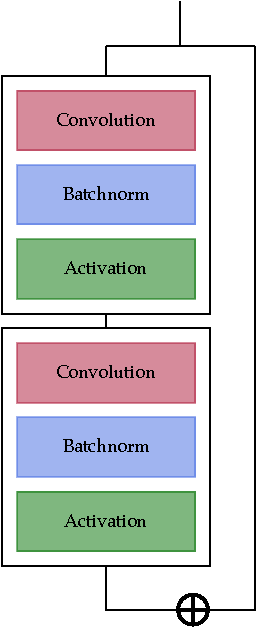
\includegraphics[width=0.45\textwidth]{machine_learning/figures/resnet}
	\caption{Resnet block}\label{fig:resnet}
\end{figure}


\section{Deep transfer learning}
\todo{do}


